\lstset{
  language=C,                % choose the language of the code
  numbers=left,                   % where to put the line-numbers
  stepnumber=1,                   % the step between two line-numbers.        
  numbersep=5pt,                  % how far the line-numbers are from the code
  backgroundcolor=\color{white},  % choose the background color. You must add \usepackage{color}
  showspaces=false,               % show spaces adding particular underscores
  showstringspaces=false,         % underline spaces within strings
  showtabs=false,                 % show tabs within strings adding particular underscores
  tabsize=2,                      % sets default tabsize to 2 spaces
  captionpos=b,                   % sets the caption-position to bottom
  breaklines=true,                % sets automatic line breaking
  breakatwhitespace=true,         % sets if automatic breaks should only happen at whitespace
  title=\lstname,                 % show the filename of files included with \lstinputlisting;
}

\section{Mérés célja}

A mérés célja a szoftverrádiók, szoftveres jelfeldolgozási technikák, valamint a kooperatív
módon működő szekunder radarok szabványos üzenetváltásának módjával való
megismerkedés.

\section{Mérés}

\subsection{Elsőfordítás}
\begin{figure}[h]
    \centering
    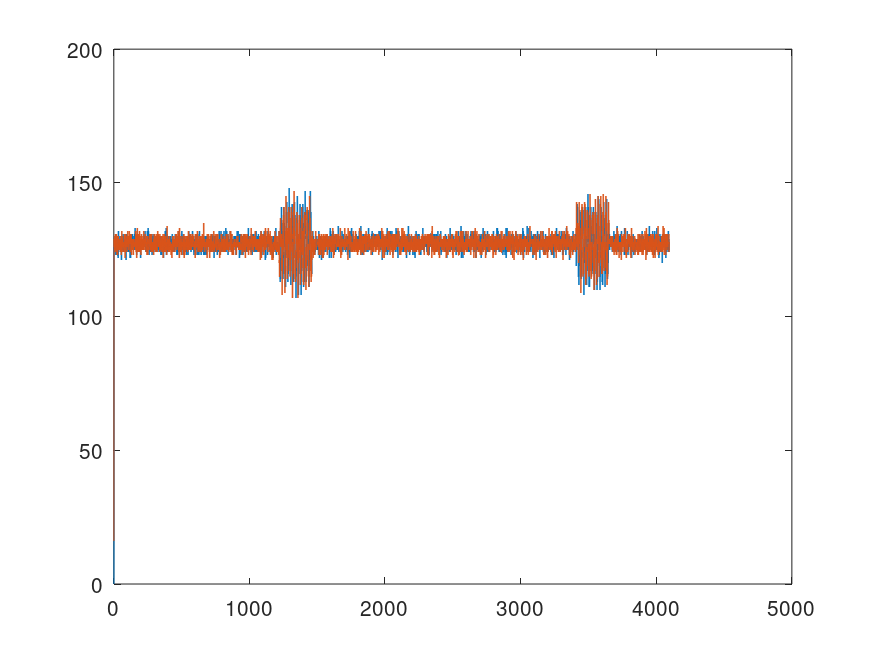
\includegraphics[width=0.9\textwidth]{../meres/result/elso_forditas.png}
    \caption{Első fordítás}
    \label{fig:first}
\end{figure}
\newpage
\subsection{Abszolút érték meghatározása}
\begin{lstlisting}
    abs_val=iq_to_abs[buffer[bix]][buffer[bix +1]];
\end{lstlisting}
\begin{figure}[h]
    \centering
    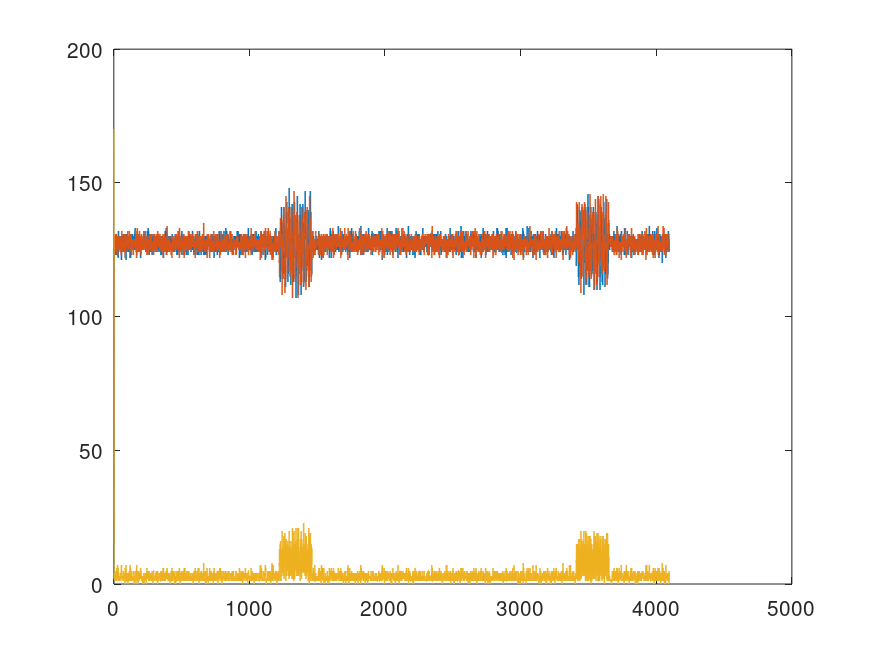
\includegraphics[width=0.9\textwidth]{../meres/result/abs_value.png}
    \caption{Abszolút érték meghatározása}
    \label{fig:abs}
\end{figure}

\newpage
\subsection{Döntési küszöb meghatározása}
\begin{lstlisting}
accumulator -= fifo[fptr];
accumulator += abs_val;
fifo[fptr] = abs_val;
fptr = fptr+1;
fptr = fptr%FIR_LEN;
\end{lstlisting}
\begin{figure}[h]
    \centering
    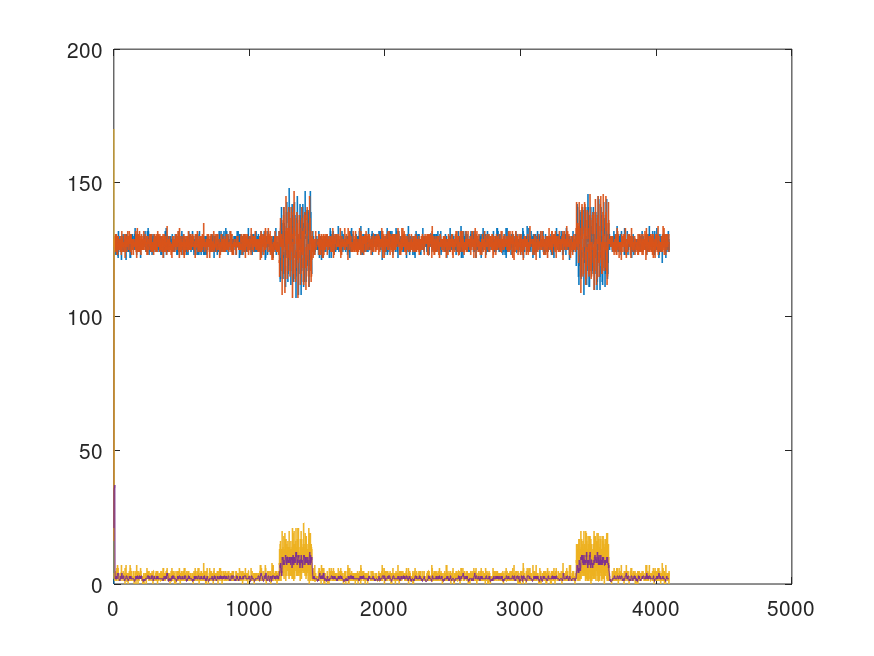
\includegraphics[width=0.9\textwidth]{../meres/result/dontes.png}
    \caption{Döntési küszöb meghatározása}
    \label{fig:deceison}
\end{figure}

\newpage
\subsection{Preamble detekció és csomag dekódolás}
\begin{lstlisting}
// Decoding
if (fifo[i] > (accumulator/FIR_LEN))
    bit = 1;
else
	bit = 0;
	// ADS-B packet search and print
	if (stm < 16)
	{
		if(bit == adsb_preamble[stm])
			stm++;
        else
			stm = 0;
    }
	else if((stm>=16)&&(stm<PCKT_LEN))
	{
		if (stm==16) printf("*");
		if ((stm%2)==0)
		{
			printf("%d",bit);
			hex=hex|bit;
			j++;
			if(j==8) {
                printf("%02x",hex);
				hex = 0;
				j = 0;
			}
			else hex = hex<<1;
		}
            stm++;
	}
	else
	{
		printf(";\r\n");
		stm = 0;
	}
\end{lstlisting}
\begin{figure}[h]
    \centering
    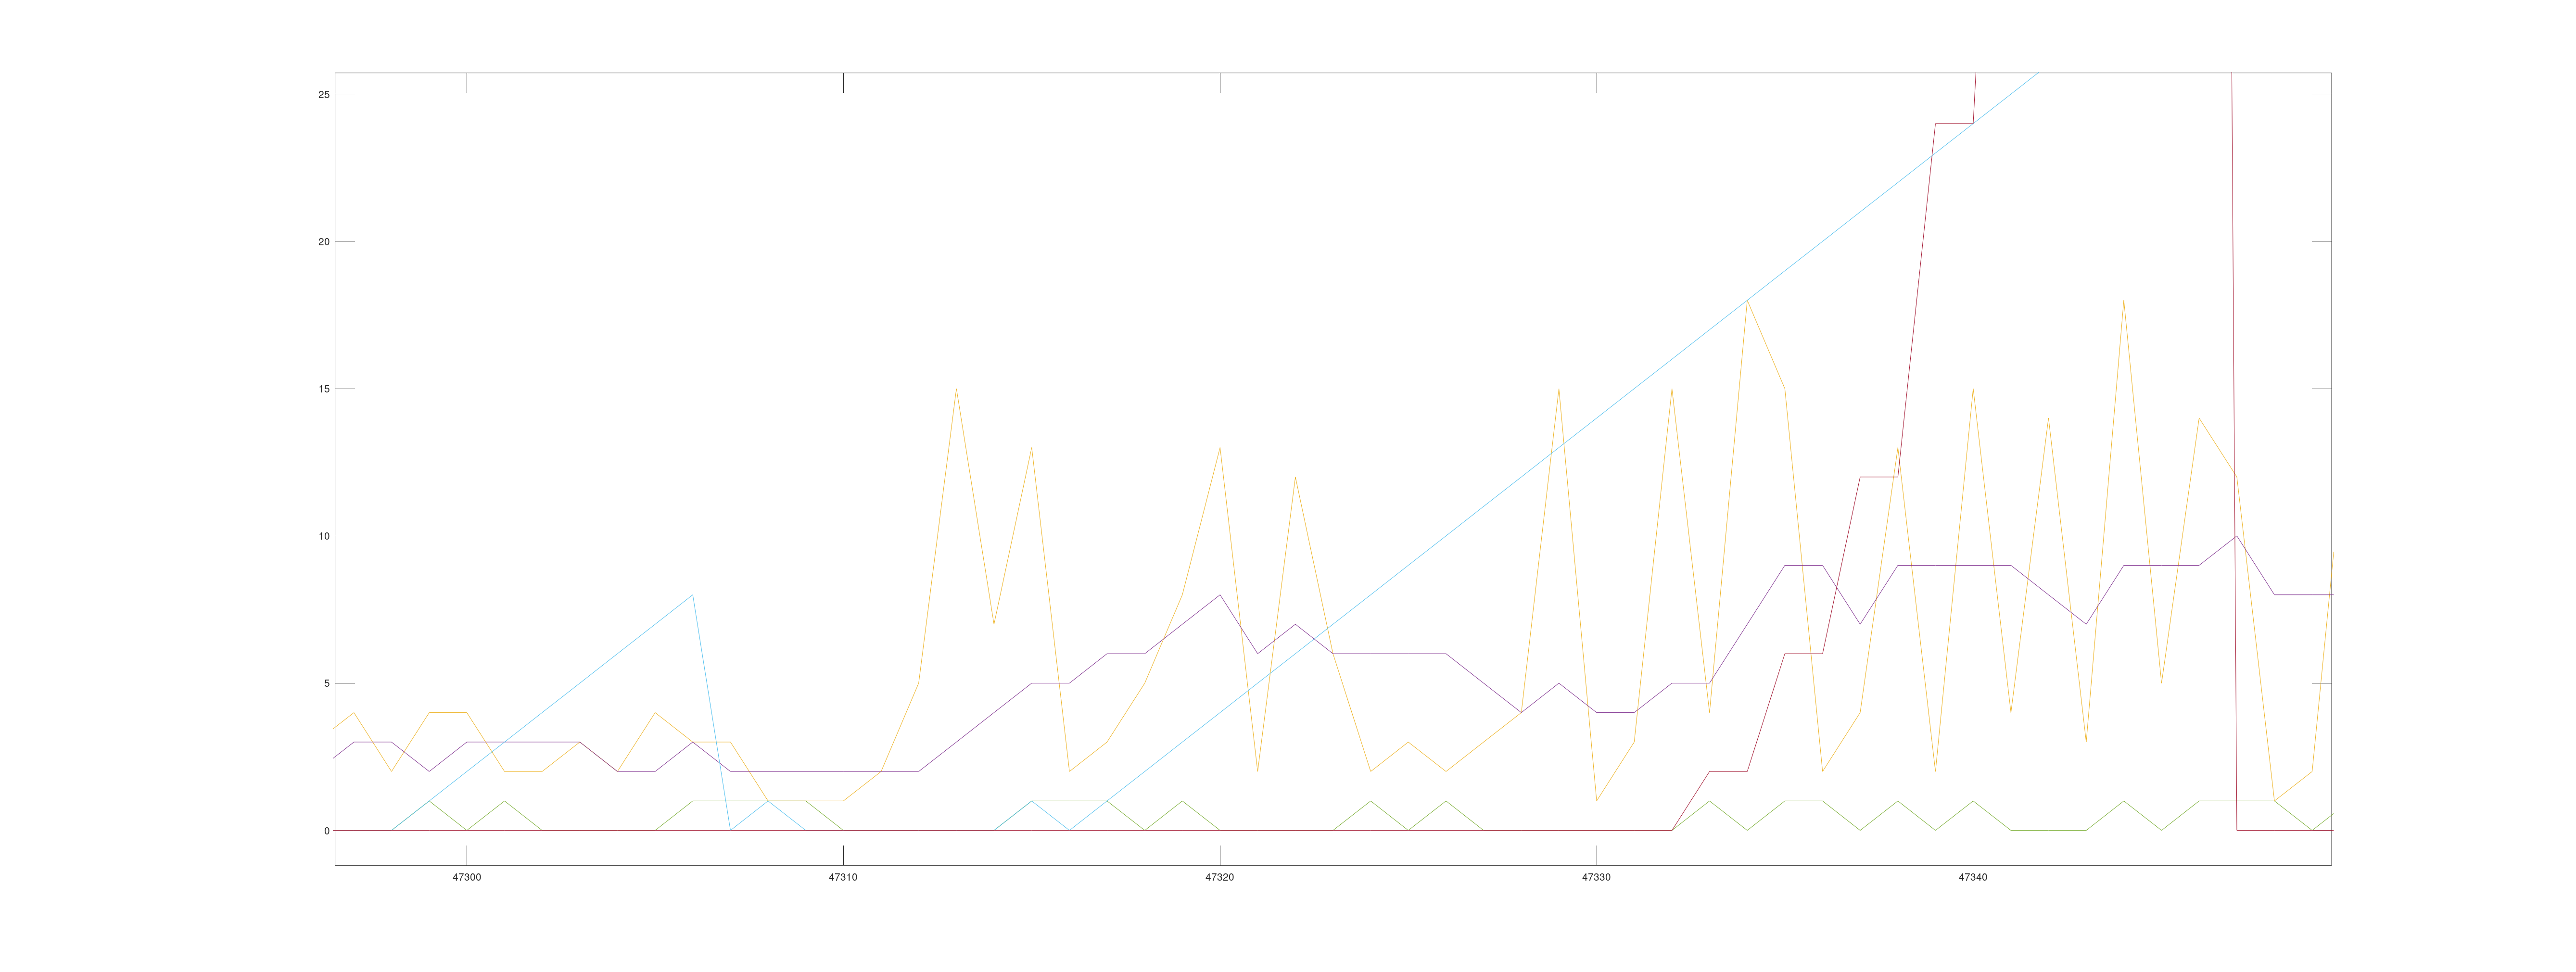
\includegraphics[width=1\textwidth]{../meres/result/preambledet_datacalc.png}
    \caption{Preamble detekció és csomag dekódolás}
    \label{fig:deceison}
\end{figure}

\newpage
\subsection{Dekódolt csomagok}
\begin{lstlisting}
*c1170812c5448254874a21bfb2c8;
*cc4687105d7339a7250192009305;
*9550d8b2a841cce0ac501a0ed2c4;
*1886ad56a6b5f312860aca8c021d;
*0fd620967105a8127c5117a8ded7;
*069431ec11059a3781923a225998;
\end{lstlisting}

\subsection{Kiértékelés}
A mérés sikeresnek tekinthatő mert, a mérés során sikerült az adsb jelet demodulálni illetve a csomagokat is megfelelően dekódolni.\\
\\
A mérés forráskódja illetve a mérés során használt adat fájlok illetve a mérési eredmények a következő linken elérhetőek: \url{https://github.com/kozdavaa/adsb_meres}
